%
\section{Foundations}
The two basic building blocks of all that is done in Nektar++ are the concepts of Points and of a Basis.  The Point objects denote positions
in space, either on compact domains (normally $[-1,1]^d$ where $d$ is the dimension in a reference domain mapped to world-space) 
or periodic domains such as $(0,2\pi]$ (i.e. in the case of points used in Fourier expansions).   
The Basis objects denote functions (e.g. polynomials) evaluated at a given set of points.

We rely heavily on the concept of ``managers'', and this concept has its start right here in Foundations.  When we started our development of
{\nek}, we realized that a pure encapsulation strategy for Expansions would consist of every expansion holding a pointer to the basis (of some sort)
that was used to specify it, and then correspondingly the basis pointing to a collection of points at which it was evaluated.  From the computer
science perspective, this is all very reasonable except for the fact that there are many cases in spectral/$hp$ element expansions in which
multiple elements use the same reference space basis functions, and correspondingly those basis functions are often evaluated at the same
set of points (quadrature points).  This led us to the conclusion that if we were going to have a code that could run over large number of elements
(at the time tens of millions) without excessive memory usage, we would have to try to avoid as much of this duplication as possible.  This led us
to introduce to {\nek} two important computer science tools:  {\em smart pointers} and {\em managers} (i.e. a factory pattern).  

{\em Smart pointers} were originally introduced as an add-on from the {\em Boost} library and later directly incorporated into {\nek} when
they were natively handled by C++11.  With the tradition view of pointers, one has a variable that holds an address that points to a place in memory.  Typically, in type-safe programming, the way this memory is to be interpreted is denoted by the type of pointer:  a double pointer (i.e. double*) is a pointer
to memory that should be interpreted as a double.  The downside of this traditional view occurs when multiple pointers all point to the same place in memory.  The question then arises: which pointer (or more properly which thread of control containing a pointer) is responsible for deleting the memory
when it is no longer needed?  Again, in the traditional view that each pointer points to unique memory and hence when the memory is not longer needed
the memory can be released no longer is viable when multiple pointers all point to the same piece of memory.  This probably was solved with the
invention of the smart pointer, an object that is wrapped up to look like a pointer, and yet contains a reference counter within it.  When a smart
pointer is initiated and memory is originally assigned to it, the reference counter is incremented.  As more and more references to the piece of memory
are created, the increment counter continues to increase.  As pointers go out of scope and are longer valid, the increment is decremented.  Only
when all the references to a particular piece of memory are removed can a {\em free} (i.e. delete) operation be accomplished.   The introduction
of smart pointers into C++ and into {\nek} were particularly advantageous to us as they allowed us to have lots of different elements, expansions, etc.
point to the same fundamental data structure in memory (for instance, a Basis object evaluated at a particular set of points) without having to worry
about improper deallocation or memory leakage due to pointer mishandling.

The second important feature we exploited within the redesign of {\nek} was the idea of {\em managers} (i.e. a factory pattern).  You will
see this use of the term manager throughout {\nek}.  For us, a manager has the following characteristics:  it expects as input a {\em key}, which
gives the manager sufficient information to know the object for which it is receiving a request.  If the manager already has one of those objects
in storage, it passes back a (smart) pointer that that object.  The manager itself continues to hold on to a pointer for the object (in case other
requests are made of it for that object).  If the manager does not have a copy of the requested object, then it has the ability to generate 
the object ``on the fly'' and store it for future use.  This last component of the manager is the factory feature that we mentioned earlier -- a
manager has registered with it a collection of methods that know how to generate the various objects that might be requested of it.

Based upon these two concepts: two fundamental managers that exist at this level of the library are the PointsManager and the BasisManager.
These are contained within ManagerAccess.h/cpp, and are defined as singletons and defined globally 
so that they can be accessed throughout {\nek}. Within these files you will find the RegisterCreator method 
calls that link particular Create methods with various keys.  Only in rare cases will these
every need to be modified, and only infrequently possibly added to (if additional Points or Basis information is given).


\subsection{Points}
One of the two primary data structures in this directory is Points.  
A points object consists of a PointsKey and then extra information needed
to facilitate various operations at points.  The basic layout of the data structure is shown in Figure \ref{foundations:pointsclass}.

\begin{figure}[htb]
\centering
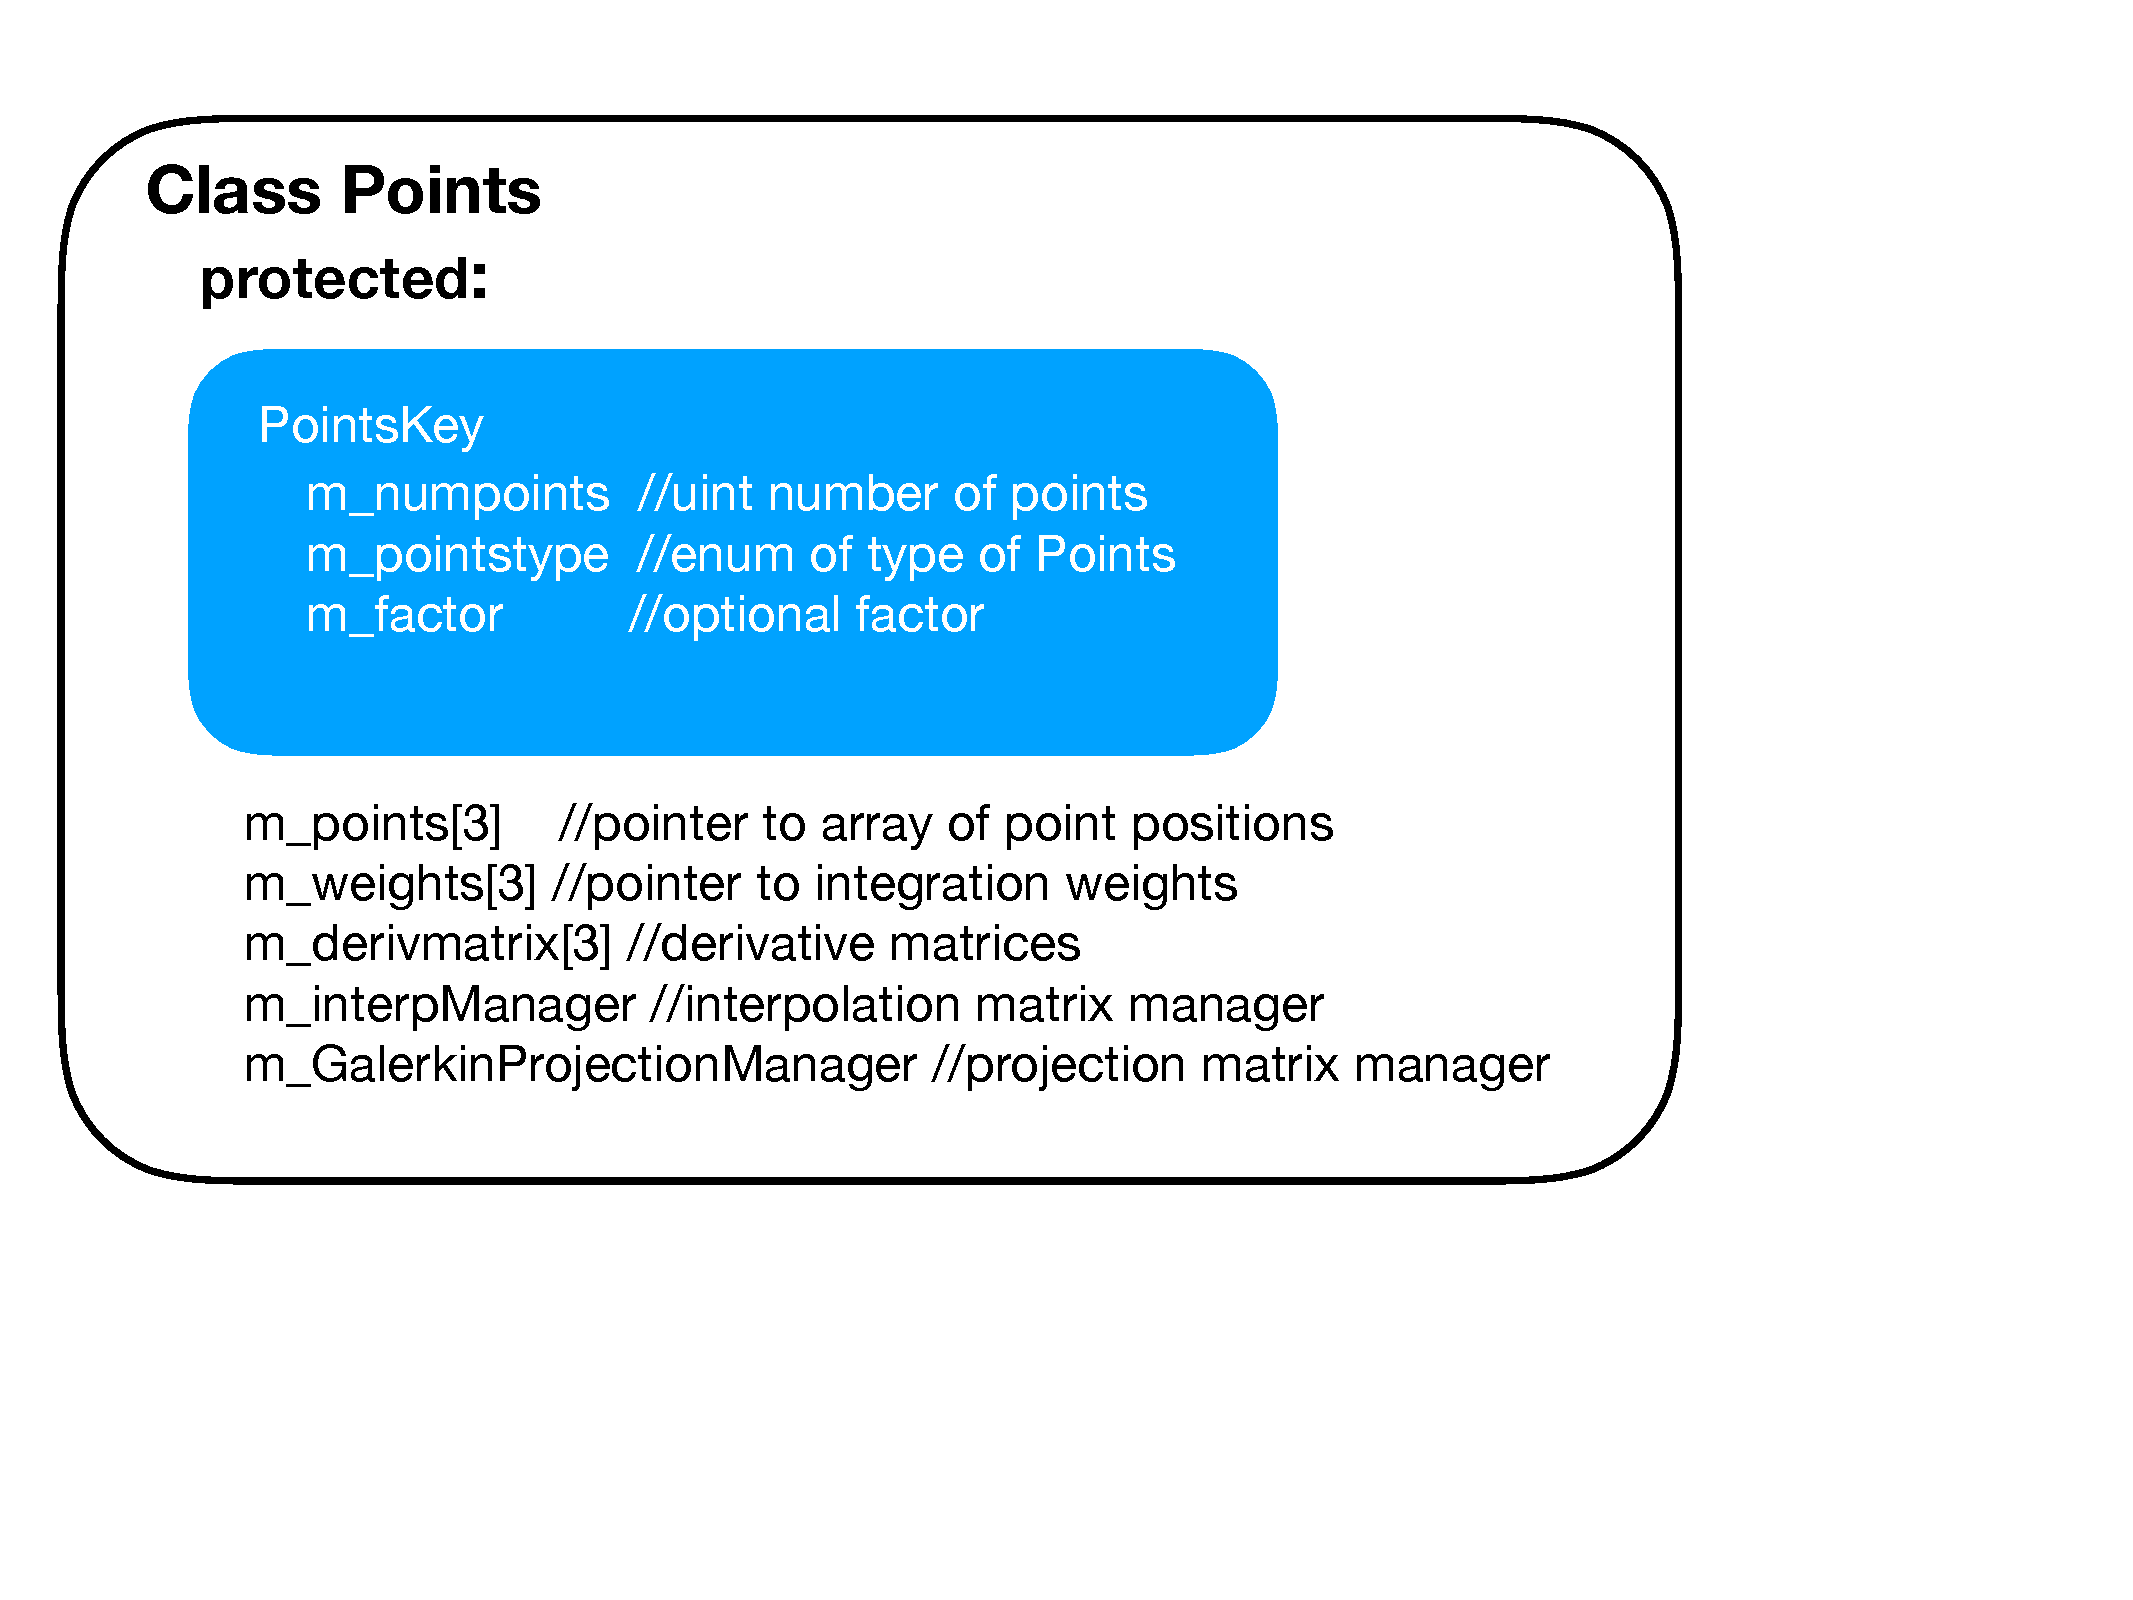
\includegraphics[width=4in]{img/pointsclass.pdf}
\caption{The basic Points class data object.  It consists of a PointsKey (used by a PointsManager) and various other data members needed for point operations.}
\label{foundations:pointsclass}
\end{figure}


The PointsKey object has three basis data members: the number of points, an enum specifying the point distribution, and a optional
scaling factor.  In almost all of {\nek}, only the first two are needed to uniquely specify a collection of points.  The latter variable was
added as part of the extensions of {\nek} to accommodate NekMesh.  As stated above, if you pass a PointsKey to a PointsManager
you will receive back a pointer to a Points object with its various data members populated, among them a PointsKey identifier for the
object.  As can be seen by the diagram, the Points object has a collection (array) of three pointers to point positions.  These three
array pointers allow Points objects to point to 1D, 2D or 3D point positions.  Corresponding to the dimension and associated with each
point position is a weight associated with integration.  This was done to facilitate both non-tensor product and tensor product constructions. 
To demonstrate non-tensor product constructions, consider if you were 
to be dealing with a 2D point set that is natively 2D (that is, not based upon tensor product construction such
as the Electrostatic Points), then the number
of points in the PointsKey would be the size of each array associated with \verb+m_points+, and only one of the \verb+m_weight+ 
arrays (associated with \verb+m_weight[0])+ would be valid such at:

\[
\int_{\Omega_{2D}} f(x_{0},x_{1}) \, dx_0\,dx_1 \approx \sum_{i=0}^{numpoints-1} \omega_i f(z_{0,i},z_{1,i})
\]

\noindent where $z_{0,i}$ and $z_{1,i}$ denote the points associated with \verb+m_points[0][i]+ and \verb+m_points[1][i]+ respectively.
The weights in this case are calculated by routines found in NodalUtils via forming a Vandermonde system, solving for Lagrange
basis functions that pass through a particular set of points, and then integrating those basis functions to obtain weights. 
This operation is done sufficiently often that we will try to spell it out after the Fekete Point paragraph below.  

If one is dealing with a tensor product constructed 2D nodal point set, one would have:

\[
\int_{\Omega_{2D}} f(x_{0},x_{1}) \, dx_0\,dx_1 \approx \sum_{i=0}^{numpoints-1} \left[ \sum_{j=0}^{numpoints-1} \omega_i \omega_j f(z_{0,i},z_{1,j})\right]
\]

\noindent where $z_{0,i}$ and $z_{1,i}$ denote the points associated with \verb+m_points[0][i]+ and \verb+m_points[1][i]+ respectively
and $\omega_i$ and $\omega_j$ are the weights associated with the two coordinate directions respectively.  The tensor product
construction above was implemented in {\nek} assuming we would create derived nodal point sets for quadrilaterals and hexahedron; however,
throughout much of {\nek}, we use the tensor product forms explicitly by specifying 1D point sets in the different directions as needed.
This particular point will become more apparent when you get to reading the Chapter on StdRegions (Chapter \ref{chap:stdregions}).  You will
encounter, for instance, that a Standard Quadrilateral Expansion (StdQuadExp) requires two 1D Point objects denoting the two 
coordinates for integration.  In this case, the number of points and number of weights match up per direction.


\paragraph{Electrostatic Points: }

The Electrostatic (Nodal) Points on the triangle and tetrahedron are based upon the work 
of Hesthaven \cite{Hesthaven98}.  They are an attempt to find the minimizer of a potential energy function based upon
an electrostatic point source analogy, and provide points that correspondingly have low Lebesgue constant.  The point positions
as given in the paper are stored in the files NodalTriElecData.h and NodalTetElecData.h.  
Hesthaven uses a condensed format for the nodal positions which
rely on the symmetries of the points (if you count the points in the file, you will see that fewer points are given than are needed
to span the polynomial space.  For example, for degree one, a single point it given.   This point along with its three-fold symmetries
represent all three points needed to support the linear space).   The routine \verb+CalculatePoints()+ expands the condensed 
format of the points to the full set based upon the one, three (a and b denoting two types of three-symmetries) 
and six symmetries.  Note that the ordering of the nodes
expanded from the file does not respect any particular geometric ordering, so we reorder the points using \verb+NodalPointReorder2d()+,
which reorganizes the points in vertex points, edge points, and then interior points (i.e. a geometric decomposition that aligns more
naturally with the way we organize nodes/modes within {\nek}).  In Figure \ref{foundations:nodeordering} we show an example
of this reordering done for the points needed for expressing a total degree three expansion over a triangle.

\begin{figure}[htb]
\centering
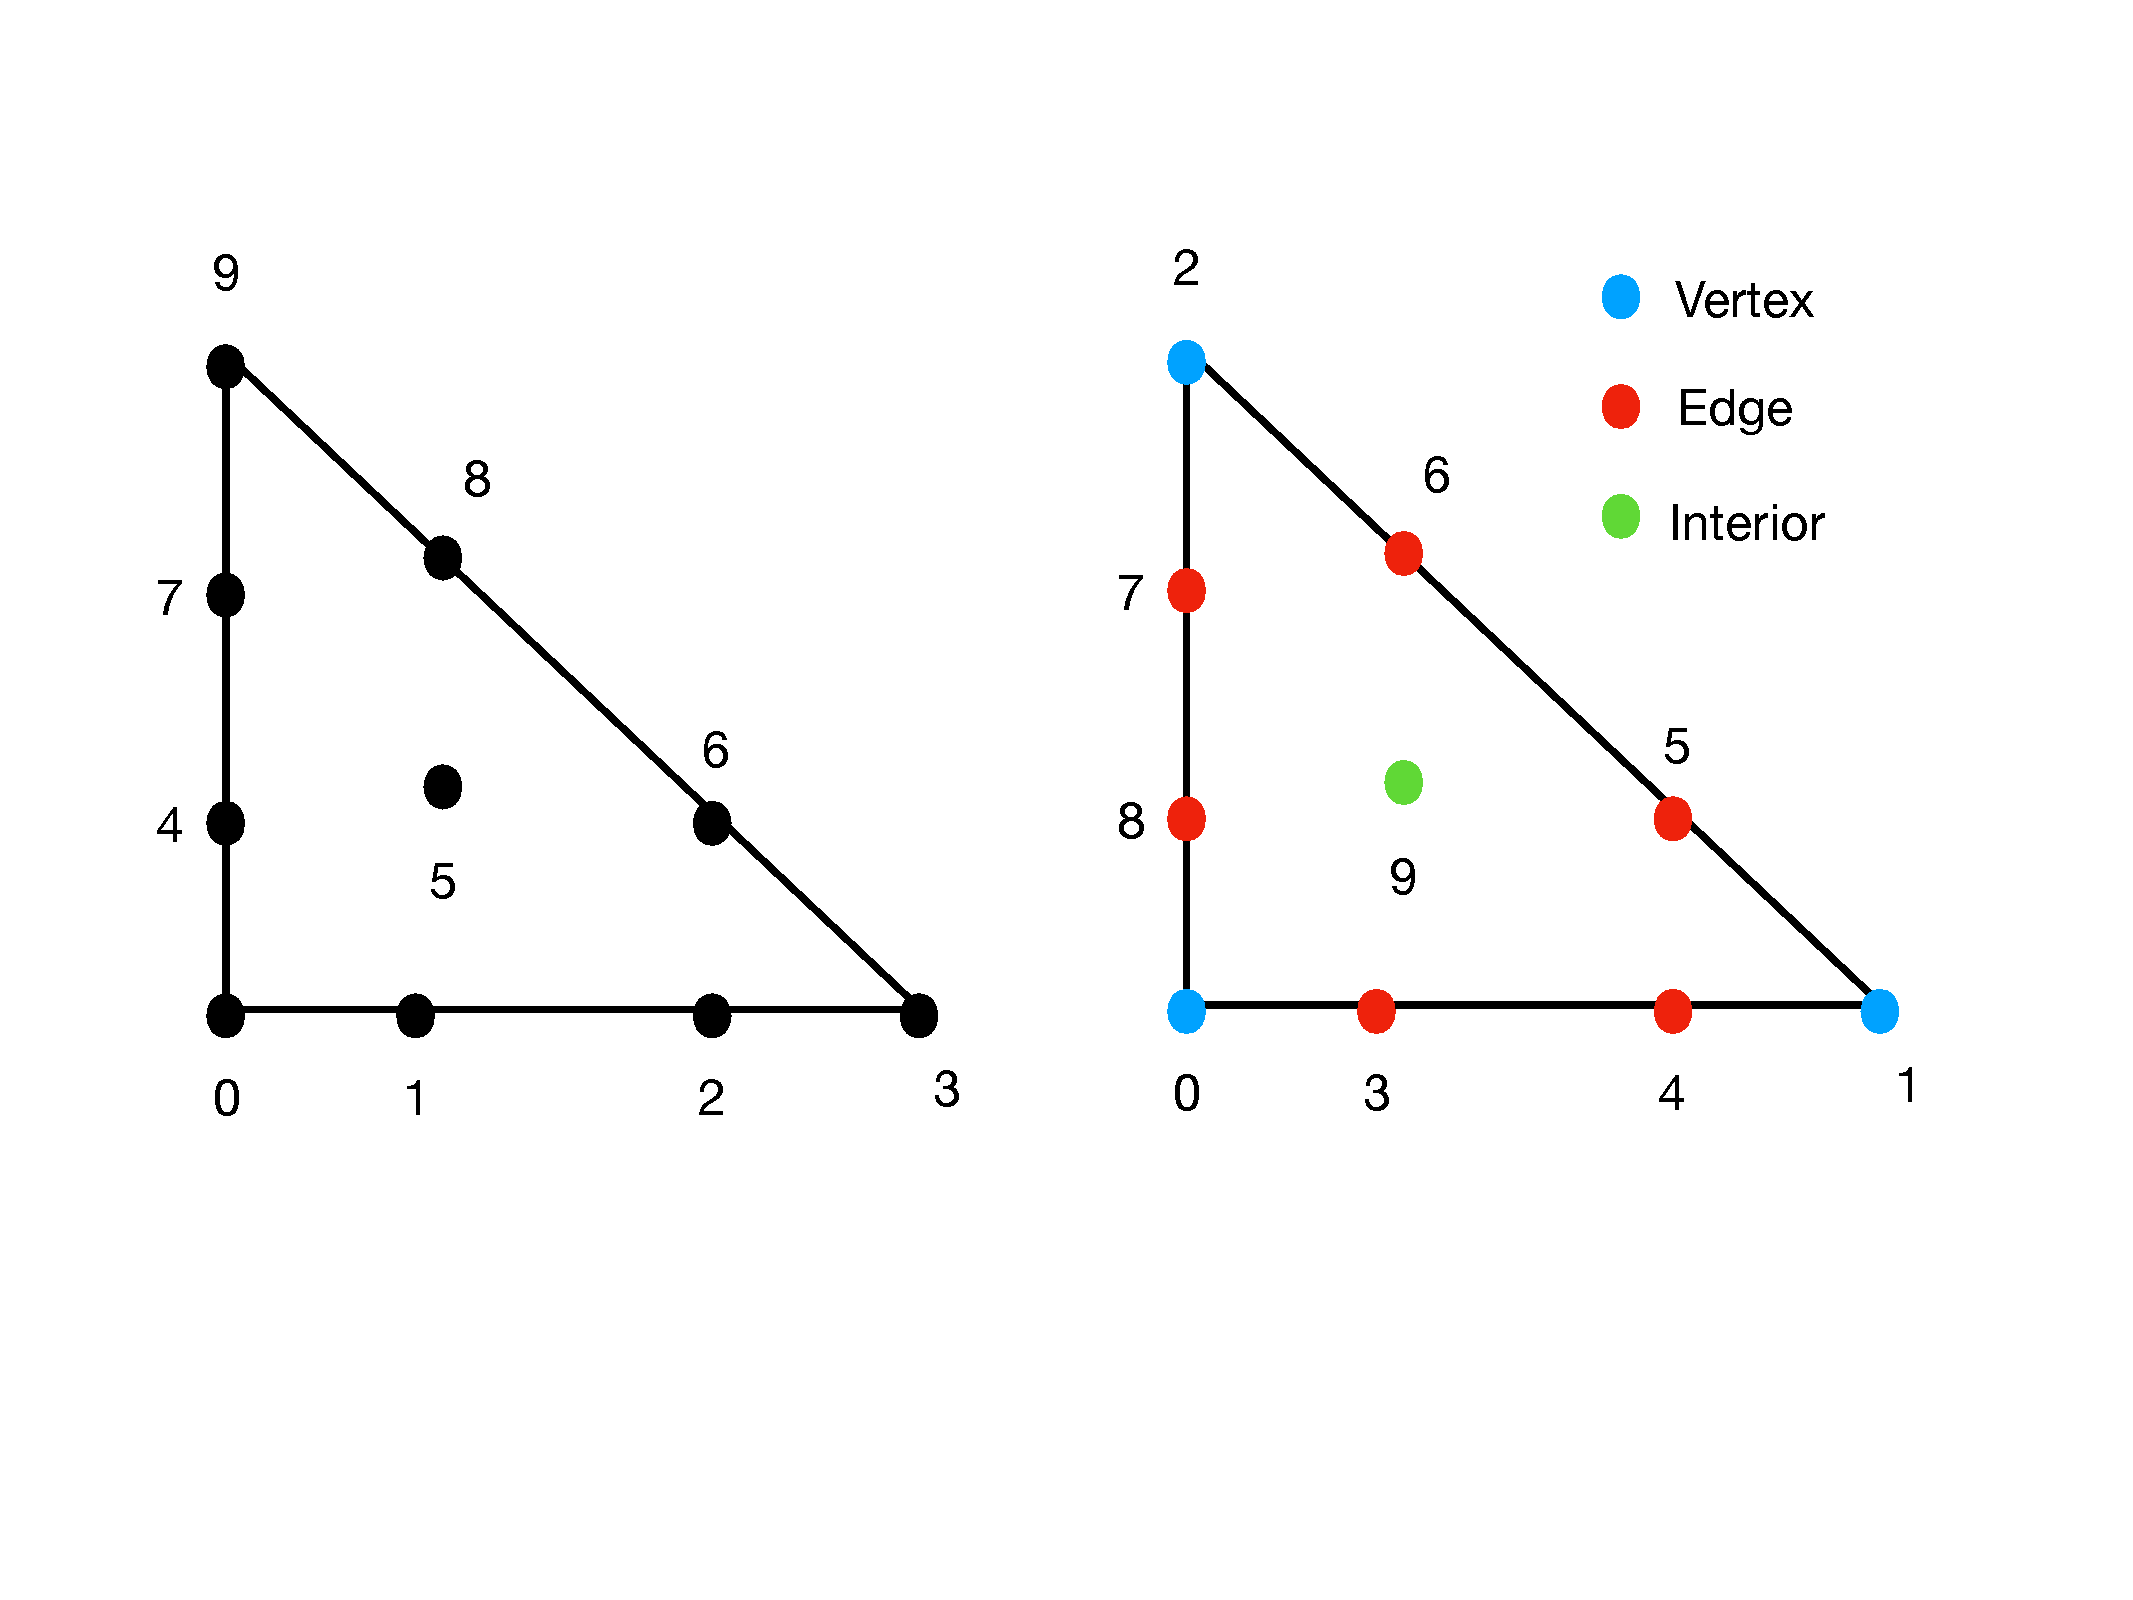
\includegraphics[width=4in]{img/nodeordering.pdf}
\caption{Example of how nodes are reordered to meet a geometric ordering.  On the left, we show the nodal positions that would
be used for building a total degree three polynomial space over a triangle ordered in canonical form.  On the right, we show 
the reordering of those nodes to follow a vertex, edge and interior ordering.  Note that in the case of a tetrahedron, the
ordering would be vertex, edge, face and then interior.}
\label{foundations:nodeordering}
\end{figure}


\paragraph{Fekete Points: }

The Fekete (Nodal) Points on a triangle are based upon the work of Taylor and Wingate \cite{TaylorW99,TaylorWV00},
and are an alternative nodal point distribution on both triangles and tetrahedra. 
As an alternative strategy to the one mentioned above, Taylor and Wingate explicitly attempt to find a point
distribution that minimizes the Lebesgue constant.  For their particular point set, the minimization if over
the Lebesgue function itself (not the electrostatic potential function, which can be viewed as a proxy for this function).  
The point positions as given in the paper are stored in the file NodalTriFeketeData.h and NodalTetFeketeData.h.  
Taylor and Wingate use a condensed format for the nodal positions similar to that used by Hesthaven.

\paragraph{Building Lagrange Interpolating Polynomials: }
One common operation done in both the case of the Electrostatic Points and the Fekete Points is to build the
Lagrange interpolating polynomial associated with a point set.  This is needed, for instance, for computing the integration
weights associated with a particular collection of points (as mentioned above).  This 
operation is done sufficiently often that we will try to spell it out here.  Forming the Lagrange basis functions for a particular
set of points, in particular in 2D and 3D, is non-trivial.  The most common way of arriving at a set of actionable basis functions is
to use a known basis (for which we are able to explicitly write down its form) 
and find the linear combination of those basis functions that yield the Lagrange basis.  For example, let us
assume we are dealing with the set of Electrostatic Points on a triangle.  The number of points, \verb+numpoints+, will
specify the number of ``modes'' (coefficients) we expect to find.  The total degree of the space is given by $N = \frac{(M+1)(M+2)}{2}$
where $N$ is the degree of the polynomials and $M$ is the number of points.  As an example: 
note that when $M=3$, we get $N=1$ -- that is, with three points we can support a polynomial of total 
degree one over a triangle.  Let $\phi_i$ denote a known non-interpolating basis function.  Although not
done in practice, imagine that this is, for instance, a monomial.  In 1D, this would equate to $\phi_i(x) = x^i$, and in
multiple dimensions this would equate to $\phi_i(x,y) = x^{i_1}y^{i_2}$ with some index mapping function $i=\sigma(i_1,i_2)$
that gives us an index ordering.  The total number of basis functions to span our degree $N$ space is given by $M$.
We first form the Vandermonde matrix ${\bf V}$ as follows:


\[
 {\bf V} =  \left[ {\begin{array}{cccc}
   \phi_0(x_{0,0},x_{1,0}) & \phi_1(x_{0,0},x_{1,0}) & \ldots & \phi_N(x_{0,0},x_{1,0}) \\
   \phi_0(x_{0,1},x_{1,1}) & \phi_1(x_{0,1},x_{1,1}) & \ldots & \phi_N(x_{0,1},x_{1,1}) \\
                                        & \vdots & & \\
   \phi_0(x_{0,N},x_{1,N}) & \phi_1(x_{0,N},x_{1,N}) & \ldots & \phi_N(x_{0,N},x_{1,N}) \\
  \end{array} } \right]
\]

\noindent where each row $i$ denotes the evaluation of our $N$ basis functions at a given point $(x_{0,i},x_{1,i})$.
Since we have selected the number of basis functions to be what can be uniquely resolved by our $N$ points, this matrix
is square and invertible.  The conditioning of the matrix is based upon our basis choice; hence we know that monomials 
are not a good choice beyond approximately cubics so in general we use our internal modified basis for this system.
With ${\bf V}$ now available, we can form the linear system:

\[
{\bf V}{\bf c} = {\bf b}
\]

\noindent where ${\bf c}$ is the vector of coefficients and where ${\bf b} = b_i$ is a binary vector where the $i^{th}$ entry is set to one
when finding the coefficients for the $i^{th}$ Lagrange basis function associated with a particular set of points.  For each Lagrange
basis function definition we seek to find, we update the right-hand-side vector and solve the linear system for the set of 
coefficients that denote the combination of our known basis that yields a Lagrange basis function.  Note that since this
operation (of ``inverting" this linear system) must be done for each Lagrange basis function, we can optimize our operations 
by accomplishing LU decomposition on ${\bf V}$ first, which can be done in $\mathcal{O}(N^2)$ operations, and then
each solution for the coefficient vector can be done in $\mathcal{O}(N)$ operations through backsolves.

\paragraph{Finding Integration Weights: }
When the points are related to Gaussian quadrature, the array \verb+m_weights+ will contain
the appropriate Gaussian quadrature weights computed using point and weight routines found in Foundations (our polymath
library functions).  In the case of weights associated with points sets that do not lie at the zeros of Jacobi polynomials, 
we must compute the weights directly based upon Lagrange interpolation through those points.  Although this can
be done in general for any point distribution, we will focus here on evenly-spaced points (note that when one
applies this approach to Chebyshev points, one arrives at Clenshaw-Curtis quadrature \cite{ClenshawC}).
Within {\nek}, given evenly-spaced points on the interval $[-1,1]$ -- if only one point is given,
then the weight is set to $2.0$ denoting a midpoint integration rule; otherwise, the weights are given by
the following expression:

\[
w_j = \int_{-1}^1 \ell_j(\xi)\, d\xi
\]

\noindent where $\ell_j(\xi)$ is the Lagrange basis function defined over an evenly-spaced set of points $\xi_k \in [-1,1]$.
For 2D and 2D nodal point sets (such as Electrostatic and Fekete Points), this same procedure is used.   We first form the
Lagrange interpolating functions via the algorithm given above (using the Vandermonde system), and then for each 
quadrature weight compute the integral of that Lagrange basis function using some known quadrature rule (such as
tensor product quadrature via Duffy transformation; this point will be more easily understood after reading Chapter
\ref{chap:stdregions})




\subsection{Basis}
The second of the two primary data structures in this directory is Basis. 
A basis object consists of a BasisKey and the extra information needed
to facilitate various operations on the basis.  The basis layout of the data 
structure is shown in Figure \ref{foundations:basisclass}.  

\begin{figure}[htb]
\centering
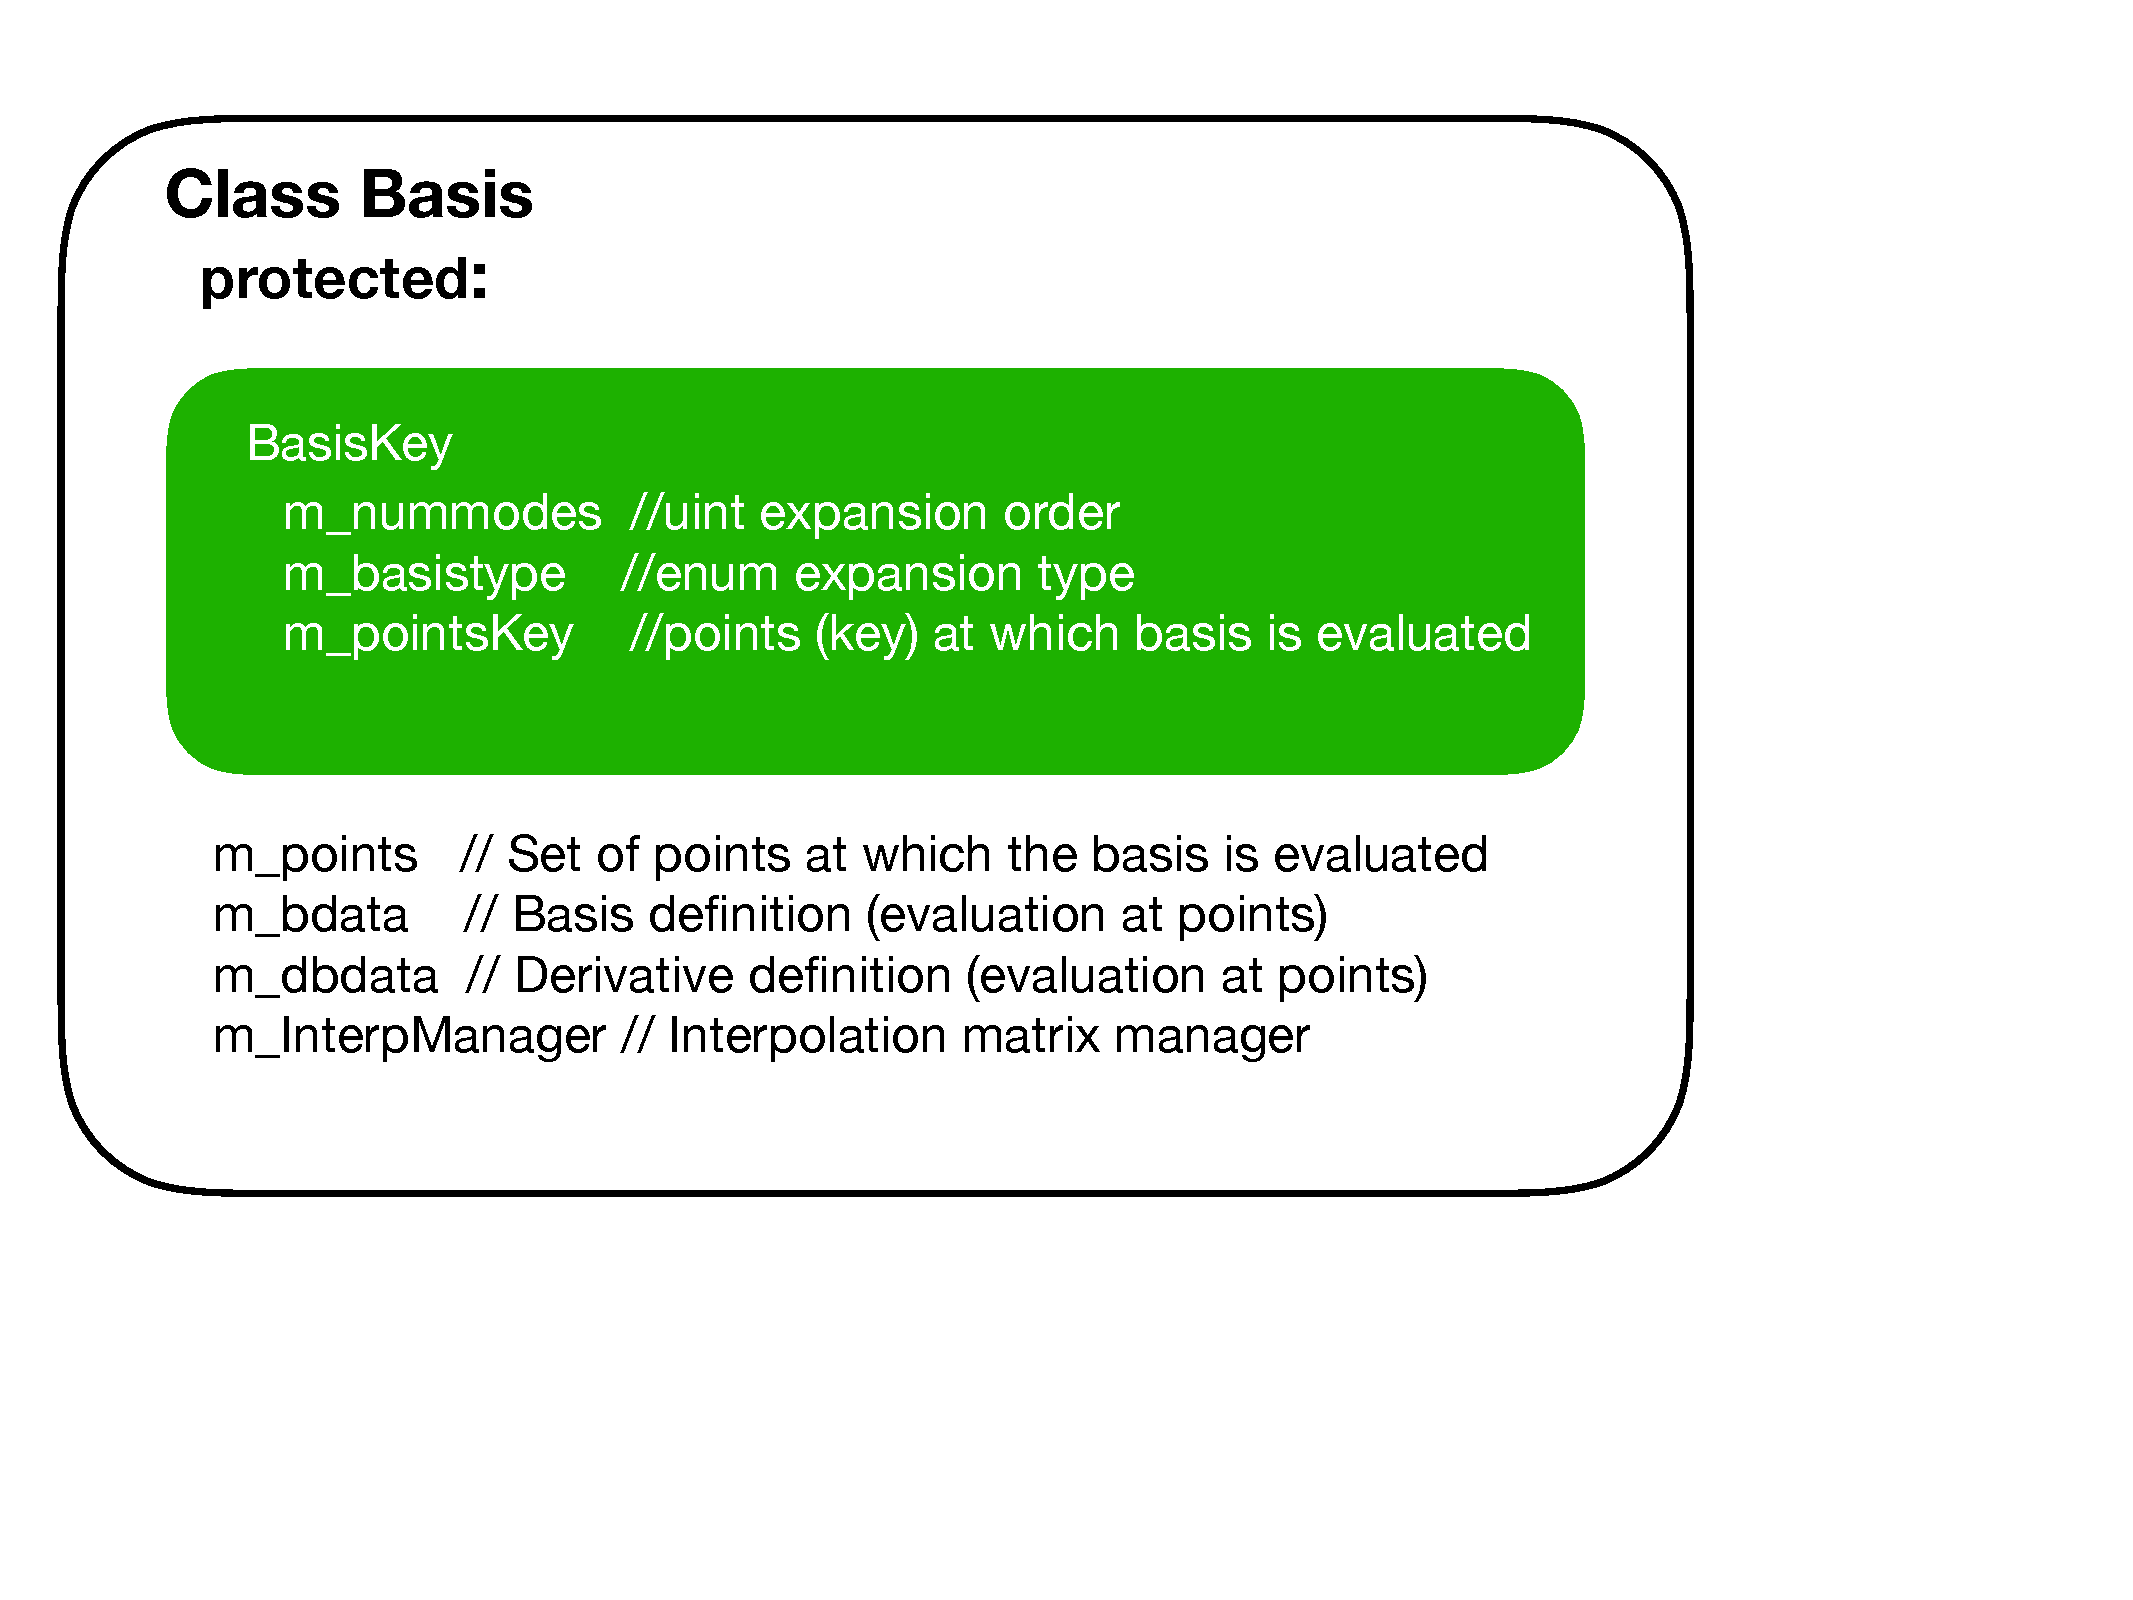
\includegraphics[width=4in]{img/basisclass.pdf}
\caption{The basic Basis class data object.  It consists of a BasisKey (used by a BasisManager) and various other data members needed for point operations.}
\label{foundations:basisclass}
\end{figure}


The Basis
object consists of a BasisKey (which in turn holds a PointsKey), 
a pointer to the positions at which the basis is evaluated and then
arrays which hold the evaluation of the basis (\verb+m_bdata+) and
the evaluation of the derivates of the basis (\verb+m_dbdata+).
The storage layout for these data structures are shown in 
Figure \ref{foundations:basisclass}.  The number of rows is given by 
the number of modes associated with a particular expansion, and the
number of columns is given by the number of points.  These arrays are stored
as contiguous memory to help avoid excessive memory hopping. 
      
\begin{figure}[htb]
\centering
\includegraphics[width=4in]{img/basismemory.pdf}
\caption{Diagram of the basic memory layout of the arrays associated with the basis and its derivatives evaluated at points.}
\label{foundations:basismemory}
\end{figure}
